\documentclass[11pt]{article}    % тип дока
\usepackage[utf8]{inputenc}   % используемые языки
\usepackage[T2A]{fontenc}   % используемые языки
\usepackage[english, russian]{babel}   % используемые языки
\usepackage[14pt]{extsizes}   % размер шрифта 14pt
\usepackage[a4paper, left=3cm, right=1cm, top=2cm , bottom=2cm]{geometry}
\usepackage{indentfirst}   % красная строка даже в первом абзаце
\usepackage{graphicx}
\usepackage{xcolor} % пакет для работы с цветами
\usepackage{amssymb}
\usepackage{amsmath}
\linespread{1.5}   % межстрочный интервал 1.5


\begin{document}

\begin{titlepage}
    
\includegraphics[scale = 0.43]{alf4.JPG}
    \\

НАПРАВЛЕНИЕ 03.03.01 Прикладные математика и физика
\par ПРОФИЛЬ Теоретическая Физика\\

\begin{center}
\begin{bf}
     ЗАДАНИЕ\\ 
     о прохождении практики по получению профессиональных умений и опыта профессиональной деятельности 
\end{bf}
  


студента Кононова Александра Михайловича \\

Курс 2 Группа 201
\end{center}

Форма обучения: очная \\
Сроки прохождения практики с 01.07.2024 по 14.07.2024 \\
Форма представления на кафедру выполненного задания: 
отчет в письменной форме\\
Дата выдачи задания: 01.07.2024\\
Задание для прохождения практики по получению профессиональных умений и опыта профессиональной деятельности: Нахождение условия параметрического резонанса в системе с периодическим $\delta$-образным потенциалом. \\
С заданием ознакомлен \\
 
Оценка \\
Руководитель практики Аверкиев Н.С\\
(Ф.И.О. полностью, должность, звание, подпись).

\end{titlepage}

\begin{titlepage}


\includegraphics[scale = 0.43]{alf4.JPG}

\

\

\

\

\

\

\begin{center}
    {\bf ОТЧЕТ по практике по получению профессиональных умений и опыта профессиональной деятельности}

    {\bf Весенний семестр 2023/2024 учебного года}

    {\bf Тема: Нахождение условия параметрического резонанса в системе с периодическим $\delta$-образным потенциалом.}

\end{center}

    {\bf Студент: Кононов Александр Михайлович}

    {\bf Руководитель практики: Аверкиев Никита Сергеевич}

    {\bf Должность, звание:}

    {\bf Оценка:}

\end{titlepage}

\tableofcontents
\newpage

\section{Введение}
\subsection{Актуальность}
Параметрический резонанс — это явление, при котором колебательная система начинает усиливаться при периодическом изменении параметров тех элементов колебательной системы, в которых сосредоточена энергия колебаний. Введение периодического дельта-образного потенциала добавляет дополнительную сложность к исследованию этого явления, позволяя изучить, как такие особенности потенциала влияют на поведение системы, включая условия возникновения резонанса, его интенсивность и устойчивость.
Параметрический резонанс в системах с дельта-образным потенциалом может найти применение в современных технологиях, например, в разработке новых типов резонаторов, сенсоров или фильтров. Понимание поведения таких систем помогает в создании устройств, которые могут адаптивно изменять свои свойства в зависимости от внешних воздействий.
%{\color{blue} Так окрашивается текст}
\subsection{Цель и задачи практики}

{\bfЦель:} 

Получить условие на параметры колебательной системы с $\delta$-образным потенциалом для возникновения параметрического резонанса.
\\

{\bfЗадачи:} 
\begin{itemize}
    \item Найти коэффициент прохождения волны через 1 $\delta$-образный потенциал
    \item Найти коэффициент прохождения волны через 2 $\delta$-образных потенциала
    \item Найти условие на параметры системы для возникновения параметрического резонанса в колебательной системе за счет двойного $\delta$-образного потенциала
\end{itemize}


\newpage

\section{Ход выполнения задания}

\subsection{Задача с одним $\delta$-образным потенциалом}
Уравнение описывающие волну в среде с некоторым потенциалом имеет вид:
\begin{equation}
    C^2(x; t) U''(x; t) = \ddot{U}(x; t)
\end{equation}
В нашем случае потенциал от времени не зависит и представляет собой лишь $\delta$-функцию, и решение мы будем искать в виде $U(x; t) = Ae^{i(kx-\omega t)}$, а значит уравнение принимает вид:
\begin{equation}
    C^2(x) U''(x) = \omega^2 U(x)
\end{equation}
Записав потенциал в явном виде получаем уравнение:
\begin{equation}
    U''(x) - k_0^2 \cdot a\delta(x) \cdot U(x) = 0
\end{equation}
Где $k_0 = \frac{\omega}{C_0}$.
\begin{center}
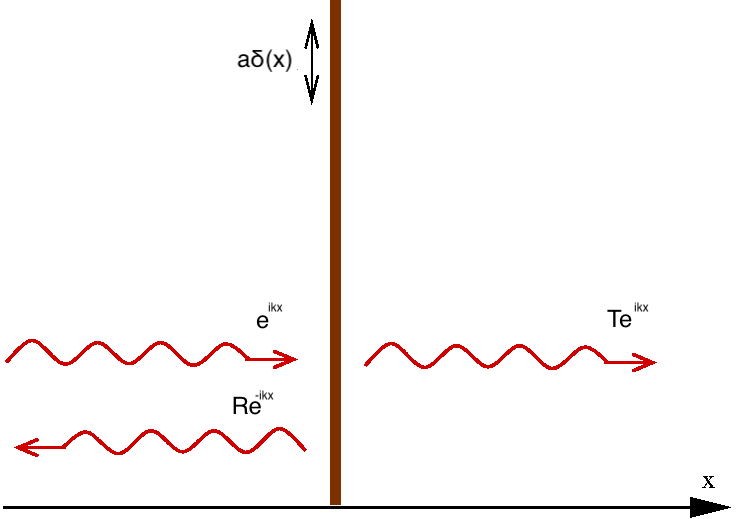
\includegraphics[scale = 0.6]{Deltapot.png}
\par
    \underline{Рисунок 1}: Прохождение волны через $\delta$-образный потенциал
\end{center}
Будем искать решение в двух областях.
В первой области в виде $U(x) = e^{ik_0x} + Re^{-ik_0x}$, во второй $U(x) = Te^{ik_0x}$.
Условия на границе двух областей такое:
\par 1) Непрерывность U(0)
\par 2) Условие на скачёк производной: $U_{x=0+}' - U_{x=0-}' + k_0^2 a \cdot U(0) = 0$
\par Составив и решив систему уравнений - получаем значения $R$ и $T$:
\begin{equation}
    \begin{cases}
        1 + R = T
        \\
        ik_0 - ik_0R - (ik_0T) + k_0^2 a T = 0
    \end{cases}
\end{equation}
Получили:
\begin{equation}
    \begin{cases}
        R = \frac{-i\frac{ka}{2}}{1+i\frac{ka}{2}}
        \\
        T = \frac{1}{1+i\frac{ka}{2}}
    \end{cases}
\end{equation}

\subsection{Задача с двумя $\delta$-образными потенциалами}
%\newpage
В этой задачи условия похожи, однако теперь в пространстве на расстоянии $b$ друг от друга разположены 2 $\delta$-образных потенциала одинаковой величины $a$.
\par
\begin{center}
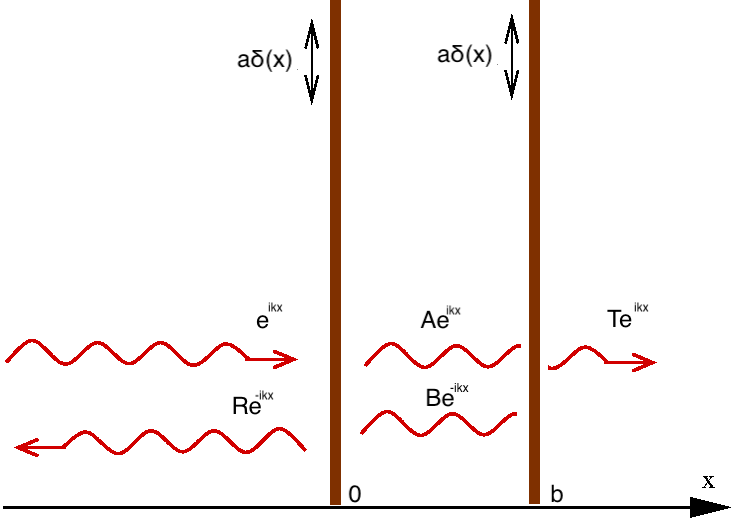
\includegraphics[scale = 0.55]{Deltapot1.png}
\par
    \underline{Рисунок 2}: Прохождение волны через 2 $\delta$-образных потенциала
\end{center}
\par Решение же теперь будем искать в 3 областях:
\begin{equation}
    \begin{cases}
        U(x) = e^{ik_0x} + Re^{-ik_0x} & x<0
        \\
        U(x) = Ae^{ik_0x} + Be^{-ik_0x} & 0<x<b
        \\
        U(x) = Te^{ik_0x}& x>b
    \end{cases}
\end{equation}
А граничных условий теперь будет 4, по 2 на каждую границу областей:
\begin{equation}
    \begin{cases}
        U_{x=0+} - U_{x=0-} = 0 & \text{, непрерывность в $0$}
        \\
        U_{x=0+}' - U_{x=0-}' + k_0^2 a \cdot U(0) = 0 & \text{, скачёк производной в $0$}
        \\
        U_{x=b+} - U_{x=b-} = 0 & \text{, непрерывность в $b$}
        \\
        U_{x=b+}' - U_{x=b-}' + k_0^2 a \cdot U(b) = 0 & \text{, скачёк производной в $b$}
    \end{cases}
\end{equation}
Получаем следующую систему уравнений на амплитуды волн:
\begin{equation}
    \begin{cases}
        1 + R = A + B % & \text{, непрерывность в $0$}
        \\
        ik_{0}A - ik_{0}B - (ik_0 - ik_0R) + k_0^2 a (1 + R) = 0 % & \text{, скачёк производной в $0$}
        \\
        Ae^{ik_{0}b} + Be^{-ik_{0}b} = Te^{ik_{0}b} % & \text{, непрерывность в $b$}
        \\
        ik_{0}Te^{ik_{0}b} - (Ae^{ik_{0}b} - Be^{-ik_{0}b}) + k_0^2 a Te^{ik_{0}b} = 0 % & \text{, скачёк производной в $b$}
    \end{cases}
\end{equation}
Решив эту систему уравнений получили выражения на коэфецииенты отражения $R$ и пропускания $T$:
\begin{equation}
    \begin{cases}
        R = \frac{(cos(ik_{0}b) + 2sin(k_0b))ie^{ik_{0}b}}{k_0a(e^{2ik_{0}b}-(1 + 2i/k_0a)^2)}
        \\
        T = \frac{4}{k_0^2a^2e^{2ik_{0}b}-(k_0a + 2i)^2}
    \end{cases}
\end{equation}
Эти результаты сходятся с результатами полученными в статье [1].
\par {\color{red} Тут написать про график Т и про то что при некоторых значениях есть полное пропускание волны}
\subsection{Задача на условие возникновения параметрического резонанса в колебательной системе за счет двойного $\delta$-образного потенциала}
\par {\color{red} тут написать про параметрический резонанс, корни, оперделитель, на вещетвенность корней, на проверку корней равных еденице условие на вещественность и возникновение параметрического резонанса}

\section{Заключение}
{\color{red} тут про то что я решил задачу без теории возмущений описывая более широкий класс потенциалов которые создают параметрический резонанс}
%\newpage

\section{Список литературы}

   \begin{enumerate}
       \item Zafar Ahmed, 'Revisiting double Dirac delta potential', European Journal of Physics (March 2016)
       \item Dr Siegfried Flugge, 'Practical Quantum Mechanics', Springer (1994)
   \end{enumerate}

%\newpage
%\section{Чеклист}
% \begin{itemize}
%     \item Вспомнить и аккуратно подписать картинки
%     \item источник статья 2005 года норм не норм
%     \item титульный лист
%     \item лист задание
%     \item разобраться с отступами
%     \item
%
%
% \end{itemize}

\end{document}
